\documentclass[a4paper,11pt]{article}

\usepackage[utf8]{inputenc}
\usepackage[T1]{fontenc}
\usepackage[english]{babel}
\usepackage{geometry}
\usepackage{graphicx}
\usepackage{booktabs}
\usepackage{caption}
\usepackage{subcaption}
\usepackage{amsmath}
\usepackage{amssymb}
\usepackage{siunitx}
\usepackage{hyperref}
\usepackage{cleveref}
\usepackage{float}
\usepackage{longtable}
\usepackage{makecell}
\usepackage{xcolor}
\usepackage{listings}

\geometry{margin=1in}
\sisetup{detect-all, group-separator={,}}

\hypersetup{
    colorlinks=true,
    linkcolor=blue,
    citecolor=blue,
    urlcolor=blue,
    pdfauthor={QBER-ML Project},
    pdftitle={Quantum Circuit Attack Classification Using QAD: An Exploratory Study Toward Temporal-QBER Detection in BB84},
    pdfsubject={Machine Learning for Quantum Attack Detection}
}

\definecolor{codegray}{gray}{0.95}
\lstset{
    backgroundcolor=\color{codegray},
    basicstyle=\ttfamily\small,
    breaklines=true,
    frame=single,
    numbers=left,
    numberstyle=\tiny,
    tabsize=4
}

\title{QBER Error Detection using ML Models}
\author{QBER-ML Project}
\date{\today}
\providecommand{\keywords}[1]{%
  \par\smallskip
  \noindent\textbf{Keywords: }#1\par
}
\begin{document}

\begin{titlepage}
\centering
{\fontsize{40}{48}\selectfont \textbf{A Project Report for Eavesdropping Detection in Quantum Communication}}\\[1cm] 

\includegraphics[width=0.4\textwidth]{figures/bits_logo.png}\\[1cm] 
{\Large Birla Institute Of Technology and Science Pilani\\ Hyderabad Campus}\\[1cm] 
{\Large \textbf{Design Oriented Project \\(CS F376)}}\\[0.5cm] 

{\large Under the supervision of\\ \textbf{Prof. Nikumani Choudhury}}\\[1.5cm]

\begin{tabular}{|c|c|c|}
\hline
\textbf{Sr No.} & \textbf{Name} & \textbf{ID Number} \\
\hline
1 & ALBERT SEBASTAIN & 2023A7PS0118H \\
\hline
2 & AKSHITH VUPPALA & 2023A7PS0032H \\
\hline
3 & MAHIMA NANDANA KUNADHARAJU & 2023B4A70660H \\
\hline
\end{tabular}
\end{titlepage}

\tableofcontents
\newpage

\section{Introduction}
\label{sec:introduction}

Quantum Key Distribution (QKD) provides information-theoretic security for cryptographic key exchange, with the BB84 protocol being the most widely implemented variant. Security in BB84 relies on detecting eavesdropping through an elevated Quantum Bit Error Rate (QBER). Traditional threshold-based detection uses a fixed QBER limit (typically 11\%), above which the key is discarded. However, this approach lacks sensitivity to attack type and temporal dynamics.

The reference paper proposes a \textbf{temporal-QBER framework}: instead of a single average QBER, the sifted key is divided into windows of $W=50$ bits, producing a QBER sequence $[q_1, q_2, \ldots, q_T]$. From this sequence, 63 physics-informed features are extracted across five categories (statistical, burst/instability, spectral/temporal, basis-dependent, channel-interaction). Three classifiers (Random Forest, XGBoost, SVM-RBF) are trained on 24,000 simulated sessions (3,000 per class across 7 attacks + normal). The paper reports XGBoost achieving 88.01\% accuracy and 0.8803 macro-F1, significantly outperforming fixed-threshold (25.82\%) and CUSUM (78.99\%) baselines in binary detection.

This report documents our current implementation, which uses the \textbf{Quantum Attack Dataset (QAD)} as a proxy dataset while the BB84 temporal-QBER simulator is under development. QAD contains 1,000,000 samples of quantum circuit executions with 7 attack types (gate tampering, noise models, measurement tampering, pulse-level distortions) plus clean circuits. We evaluate the same three classifiers and provide full explainability (SHAP) and ablation analysis.

\textbf{Critical distinction:} QAD's attack classes are \textit{quantum circuit attacks} (adversary modifies circuit structure/noise), not BB84 \textit{eavesdropping attacks} (adversary intercepts quantum channel between Alice and Bob). The high accuracy on QAD (95.8\% XGBoost) is largely attributable to attack-specific simulator parameters that directly encode the attack type---a form of label leakage not present in the BB84 threat model. This report maintains this distinction throughout.

\paragraph{Contributions of this work:}
\begin{enumerate}
    \item Complete reproducible ML pipeline for QAD dataset with three classifiers
    \item Comprehensive evaluation: accuracy, macro-F1, ROC-AUC, per-class metrics, confusion matrices
    \item SHAP explainability for tree-based models identifying feature importance
    \item Leave-one-feature-group-out ablation quantifying feature group contributions
    \item Documented limitations and roadmap for BB84 temporal-QBER reproduction
\end{enumerate}
\section{Background and Related Work}
\label{sec:background}

\subsection{BB84 Quantum Key Distribution}
The BB84 protocol establishes a shared secret key between two parties (Alice and Bob) by transmitting qubits in randomly chosen bases (rectilinear $+$ or diagonal $\times$). After transmission, Alice and Bob publicly compare bases and keep only bits measured in matching bases (sifting). The Quantum Bit Error Rate (QBER) on the sifted key reveals eavesdropping: an intercept-resend attack introduces a minimum 25\% QBER.

\subsection{QBER-Based Attack Detection}
Traditional QKD systems use a fixed QBER threshold (typically 11\% for BB84 with one-way post-processing). If the observed QBER exceeds this threshold, the key is discarded. This binary decision ignores:
\begin{itemize}
    \item Temporal dynamics of errors within a session
    \item Attack-type discrimination
    \item Channel condition variations (loss, noise)
\end{itemize}

\subsection{Temporal-QBER Framework (Reference Paper)}
The reference paper introduces a temporal-QBER framework:
\begin{enumerate}
    \item \textbf{Windowing:} Sifted key divided into non-overlapping windows of $W=50$ bits
    \item \textbf{QBER sequence:} $q_t = \frac{1}{W}\sum_{i=(t-1)W+1}^{tW} (a_i \oplus b_i)$
    \item \textbf{63 features:} Five categories extracted from the QBER sequence
    \item \textbf{8 classes:} Normal + 7 eavesdropping attacks
    \item \textbf{24,000 sessions:} 3,000 per class, balanced
    \item \textbf{Models:} Random Forest, XGBoost, SVM-RBF with 5-fold CV, 10 seeds
\end{enumerate}

\subsection{Quantum Attack Datasets}
Existing quantum ML datasets include:
\begin{itemize}
    \item \textbf{QAD}: Quantum circuit attacks (gate tampering, noise, measurement tampering, pulse distortions), 1M samples, 44 features, 8 classes
    \item \textbf{HQC-2026}: Hybrid quantum-classical network intrusion, 14.69M samples, 96 features, 7 attack categories + benign
    \item \textbf{IBM Quantum Challenge datasets}: Various quantum computing benchmarks
\end{itemize}

QAD is the most directly applicable for supervised quantum attack classification but operates at the circuit level, not the QKD protocol level.

\subsection{Machine Learning for Quantum Security}
ML has been applied to:
\begin{itemize}
    \item Quantum error correction decoding
    \item Quantum state tomography
    \item Quantum device characterization
    \item Side-channel attack detection in QKD
\end{itemize}

The temporal-QBER approach is, to our knowledge, the first to apply windowed QBER sequences with physics-informed feature engineering for multi-attack classification in BB84.
\section{Dataset}
\label{sec:dataset}

\subsection{Quantum Attack Dataset (QAD)}
\label{sec:qad}

The Quantum Attack Dataset (QAD) is a synthetic dataset generated by NetsLab (UCD) using Qiskit simulations of parametrized quantum circuits under various attack conditions.

\subsubsection{Source and Licence}
\begin{itemize}
    \item \textbf{Authors:} Pasindu Udugahapattuwa, Chamitha de Alwis, Uditha Wijewardane, Madhusanka Liyanage
    \item \textbf{DOI:} \url{https://doi.org/10.34740/kaggle/ds/9778273}
    \item \textbf{Licence:} MIT (academic and research use)
\end{itemize}

\subsubsection{Generation Process}
\begin{enumerate}
    \item \textbf{Baseline circuits:} VQC, QSVM, QNN topologies; 2--6 qubits; depth 2--10; linear/circular/all-to-all connectivity
    \item \textbf{Simulation:} Qiskit AerSimulator, 1024 shots per circuit
    \item \textbf{Attack injection:} 7 attack types with randomized parameters (Table \ref{tab:qad_attacks})
    \item \textbf{Feature extraction:} 42 base features (including \texttt{circuit\_type} as categorical); after one-hot encoding \texttt{circuit\_type} (VQC, QSVM, QNN) $\to$ 45 model features; label columns \texttt{attack\_type} and \texttt{attack\_label} excluded
    \item \textbf{Balanced dataset:} 300,000 clean + 100,000 $\times$ 7 attacks = 1,000,000 samples
    \item \textbf{Unbalanced dataset:} Variable attack frequencies (also available)
\end{enumerate}

\begin{table}[H]
\centering
\caption{QAD Attack Types and Parameter Ranges}
\label{tab:qad_attacks}
\begin{tabular}{lll}
\toprule
\textbf{Attack} & \textbf{Label} & \textbf{Parameter Range} \\
\midrule
Clean (benign) & 0 & N/A \\
Swap Injection & 1 & intensity $\in$ [0.55, 0.85] \\
Gate Insertion & 2 & intensity $\in$ [0.45, 0.75] \\
Depolarizing Noise & 3 & error rate $\in$ [0.08, 0.28] \\
Amplitude Damping & 4 & damping $\in$ [0.20, 0.55] \\
Measurement Tampering & 5 & flip prob $\in$ [0.30, 0.55] \\
Pulse-Level Attack & 6 & detuning $\in$ [0.25, 0.60] \\
Thermal Relaxation & 7 & T1 $\in$ [25, 60]$\mu$s, T2 $\in$ [10, 40]$\mu$s, gate $\in$ [100, 500]ns \\
\bottomrule
\end{tabular}
\end{table}

\subsubsection{Feature Categories}
After one-hot encoding \texttt{circuit\_type} (VQC, QSVM, QNN), the 45 model features comprise 42 base features (including the original \texttt{circuit\_type} categorical column) plus 2 additional one-hot columns (since one category is dropped to avoid multicollinearity). The features group into the following semantic categories (verified from the ablation study in Section \ref{sec:ablation}):

\begin{enumerate}
    \item \textbf{Circuit Structure (12):} \texttt{n\_qubits, circuit\_depth, n\_gates\_total, n\_single\_qubit\_gates, n\_two\_qubit\_gates, gate\_density, circuit\_type\_VQC, circuit\_type\_QSVM, circuit\_type\_QNN, has\_noise\_model, gate\_ins\_intensity, tr\_gate\_time}
    \item \textbf{Output Distribution (11):} \texttt{n\_outcomes, prob\_std, prob\_max, prob\_min, prob\_range, prob\_cv, most\_common\_count, least\_common\_count, outcome\_ratio, ad\_pop\_ratio, tr\_decay\_ratio}
    \item \textbf{Entropy (2):} \texttt{entropy, normalized\_entropy}
    \item \textbf{Purity/Diversity (8):} \texttt{purity\_proxy, dp\_purity\_proxy, dp\_uniformity\_score, ad\_coherence\_factor, ad\_pop\_asymmetry, mt\_uniformity, pl\_phase\_coherence, tr\_coherence\_est}
    \item \textbf{Attack-Specific Parameters (11):} \texttt{swap\_intensity, n\_swaps, gate\_ins\_intensity, n\_insertions, dp\_error\_rate, ad\_damping\_param, mt\_flip\_prob, pl\_detuning\_mag, tr\_t1, tr\_t2, tr\_gate\_time}
    \item \textbf{Timing (1):} \texttt{exec\_time\_sec}
\end{enumerate}

\textbf{Note:} The category assignments above reflect the actual grouping used in the ablation study (Section \ref{sec:ablation}), which differs slightly from a purely semantic grouping. Notably, \texttt{has\_noise\_model}, \texttt{gate\_ins\_intensity}, and \texttt{tr\_gate\_time} are grouped under Circuit Structure by the automated grouping logic, while \texttt{ad\_pop\_ratio} and \texttt{tr\_decay\_ratio} fall under Output Distribution.

\subsubsection{Class Distribution}
For the balanced dataset (1,000,000 samples):

\begin{table}[H]
\centering
\caption{QAD Balanced Dataset Class Distribution}
\label{tab:qad_class_dist}
\begin{tabular}{lrr}
\toprule
\textbf{Class} & \textbf{Count} & \textbf{Percentage} \\
\midrule
clean & 300,000 & 30.0\% \\
swap\_injection & 100,000 & 10.0\% \\
gate\_insertion & 100,000 & 10.0\% \\
depolarizing\_noise & 100,000 & 10.0\% \\
amplitude\_damping & 100,000 & 10.0\% \\
measurement\_tampering & 100,000 & 10.0\% \\
pulse\_level\_attack & 100,000 & 10.0\% \\
thermal\_relaxation & 100,000 & 10.0\% \\
\midrule
\textbf{Total} & \textbf{1,000,000} & \textbf{100.0\%} \\
\bottomrule
\end{tabular}
\end{table}

For our experiments we used a 10,000-sample stratified subset (Table \ref{tab:our_sample_dist}).

\begin{table}[H]
\centering
\caption{Experimental Sample (n=10,000) Class Distribution}
\label{tab:our_sample_dist}
\begin{tabular}{lrr}
\toprule
\textbf{Class} & \textbf{Count} & \textbf{Percentage} \\
\midrule
clean & 3,042 & 30.4\% \\
swap\_injection & 968 & 9.7\% \\
gate\_insertion & 1,003 & 10.0\% \\
depolarizing\_noise & 1,007 & 10.1\% \\
amplitude\_damping & 996 & 10.0\% \\
measurement\_tampering & 950 & 9.5\% \\
pulse\_level\_attack & 1,030 & 10.3\% \\
thermal\_relaxation & 1,004 & 10.0\% \\
\midrule
\textbf{Total} & \textbf{10,000} & \textbf{100.0\%} \\
\bottomrule
\end{tabular}
\end{table}

\subsubsection{Limitations for BB84 Reproduction}
\begin{enumerate}
    \item \textbf{Different threat model:} Circuit-level attacks vs. QKD channel eavesdropping
    \item \textbf{No temporal dimension:} Single aggregate statistics vs. windowed QBER sequences
    \item \textbf{Label leakage:} Attack-specific parameters directly reveal attack type/intensity
    \item \textbf{No basis reconciliation:} QAD measures all qubits; BB84 uses basis sifting
    \item \textbf{No photon loss:} Fixed 1024 shots; BB84 has detection efficiency/loss
\end{enumerate}
\section{Methodology}
\label{sec:methodology}

\subsection{Data Preprocessing}
\label{sec:preprocessing}

\begin{enumerate}
    \item \textbf{Data loading:} QAD balanced CSV (1,000,000 rows $\times$ 45 columns)
    \item \textbf{Feature/target separation:} 
    \begin{itemize}
        \item Features $X$: all columns except \texttt{attack\_type}, \texttt{attack\_label}
        \item Target $y$: \texttt{attack\_label} (0--7)
    \end{itemize}
    \item \textbf{Categorical encoding:} \texttt{circuit\_type} one-hot encoded (3 columns: VQC, QSVM, QNN)
    \item \textbf{Train/test split:} 80/20 stratified, \texttt{random\_state=42}
    \item \textbf{Standardization:} \texttt{StandardScaler} fitted on training data only, applied to train and test
\end{enumerate}

\subsection{Models and Hyperparameters}
\label{sec:models}

Three classifiers matching the reference paper's selection:

\subsubsection{Random Forest}
\begin{itemize}
    \item \texttt{n\_estimators=200}
    \item \texttt{max\_depth=20}
    \item \texttt{class\_weight='balanced'}
    \item \texttt{random\_state=42}, \texttt{n\_jobs=-1}
    \item No feature scaling required
\end{itemize}

\subsubsection{XGBoost}
\begin{itemize}
    \item \texttt{n\_estimators=200}
    \item \texttt{max\_depth=10}
    \item \texttt{learning\_rate=0.1}
    \item \texttt{eval\_metric='mlogloss'}, \texttt{verbosity=0}
    \item Balanced class weighting via per-sample weights from training labels (\texttt{sklearn.utils.class\_weight.compute\_sample\_weight} with \texttt{class\_weight='balanced'})
    \item \texttt{random\_state=42}, \texttt{n\_jobs=-1}
    \item No feature scaling required
\end{itemize}

\subsubsection{SVM-RBF}
\begin{itemize}
    \item Pipeline: \texttt{StandardScaler} $\rightarrow$ \texttt{SVC}
    \item \texttt{kernel='rbf'}, \texttt{C=1.0}, \texttt{gamma='scale'}
    \item \texttt{probability=True} (for ROC-AUC)
    \item \texttt{class\_weight='balanced'}
    \item \texttt{random\_state=42}
    \item Scaling essential for SVM
\end{itemize}

\subsection{Cross-Validation}
\begin{itemize}
    \item 5-fold stratified cross-validation on training set only
    \item \texttt{StratifiedKFold(n\_splits=5, shuffle=True, random\_state=42)}
    \item Metrics: accuracy, macro-F1
    \item Preprocessing (scaler) refitted within each fold (handled by Pipeline for SVM)
\end{itemize}

\subsection{Evaluation Metrics}
\label{sec:metrics}

\paragraph{Multiclass (8-class) metrics:}
\begin{itemize}
    \item \textbf{Accuracy:} $\frac{1}{N}\sum_{i=1}^N \mathbb{1}(\hat{y}_i = y_i)$
    \item \textbf{Macro-F1:} $\frac{1}{C}\sum_{c=1}^C F1_c$ where $F1_c = 2\frac{P_c R_c}{P_c + R_c}$
    \item \textbf{Macro-Precision:} $\frac{1}{C}\sum_{c=1}^C P_c$
    \item \textbf{Macro-Recall:} $\frac{1}{C}\sum_{c=1}^C R_c$
    \item \textbf{ROC-AUC (OvR):} One-vs-Rest AUC averaged across classes
\end{itemize}

\paragraph{Binary (attack vs. normal) metrics:}
\begin{itemize}
    \item \textbf{False Negative Rate (FNR):} $\frac{FN}{FN + TP}$ --- proportion of attacks missed
    \item \textbf{False Positive Rate (FPR):} $\frac{FP}{FP + TN}$ --- proportion of normal flagged as attack
\end{itemize}

\paragraph{Per-class metrics:} Precision, Recall, F1, Support for each of 8 classes.

\subsection{Baseline Comparisons}
The reference paper compares against:
\begin{enumerate}
    \item \textbf{Fixed 11\% QBER threshold:} Binary detector, flags attack if mean QBER $> 0.11$
    \item \textbf{CUSUM detector:} Sequential change-point detection on QBER sequence
\end{enumerate}

\textbf{Note:} These baselines require temporal QBER sequences, which QAD does not provide. Our implementation includes the baseline framework (\texttt{evaluate.py}) but reports ``Requires temporal QBER feature'' for QAD experiments.

\subsection{Explainability}
\label{sec:explainability}

\subsubsection{SHAP (SHapley Additive exPlanations)}
\begin{itemize}
    \item \textbf{TreeExplainer} for Random Forest and XGBoost (exact, fast)
    \item \textbf{KernelExplainer} for SVM-RBF (approximate, slow; not computed)
    \item Background: 100 k-means samples from training data
    \item Explanation set: 500 test samples
    \item Outputs: Global mean $|SHAP|$ importance, summary bar plots, beeswarm plots
\end{itemize}

\subsubsection{Feature-Group Ablation}
Leave-one-group-out: retrain model after removing each semantic feature group.
\begin{itemize}
    \item Groups: circuit\_structure (12), output\_distribution (11), entropy\_features (2), purity\_diversity (8), attack\_specific\_params (11), timing (1)
    \item Metric: drop in accuracy and macro-F1 vs. baseline (all features)
    \item Identifies which feature categories drive performance
\end{itemize}

\subsection{Reproducibility}
\begin{itemize}
    \item All random seeds fixed (42 for data, model-specific for training)
    \item Full pipeline saved: models, scaler, feature names, class names
    \item Exact dependency versions locked in \texttt{uv.lock}
    \item Results saved as JSON for programmatic access
    \item Single-command execution via \texttt{scripts/run\_pipeline.py}
\end{itemize}
\section{Results}
\label{sec:results}

All results are from the 10,000-sample experimental subset (80/20 split $\rightarrow$ 8,000 train, 2,000 test). Cross-validation is 5-fold on the training set. Models are trained once with fixed seeds; no 10-seed averaging was performed (unlike the reference paper).

\subsection{Multiclass Classification Performance}

\begin{table}[H]
\centering
\caption{Multiclass (8-class) Classification Results on Test Set (n=2,000)}
\label{tab:multiclass_results}
\begin{tabular}{lccccc}
\toprule
\textbf{Model} & \textbf{Accuracy} & \textbf{Macro-F1} & \textbf{Macro-Prec} & \textbf{Macro-Rec} & \textbf{ROC-AUC (OvR)} \\
\midrule
XGBoost & 0.9575 & 0.9463 & 0.9461 & 0.9466 & 0.9976 \\
Random Forest & 0.9545 & 0.9421 & 0.9423 & 0.9432 & 0.9972 \\
SVM-RBF & 0.7885 & 0.7582 & 0.7792 & 0.7625 & 0.9746 \\
\bottomrule
\end{tabular}
\end{table}

\begin{table}[H]
\centering
\caption{5-Fold Cross-Validation Results on Training Set (n=8,000)}
\label{tab:cv_results}
\begin{tabular}{lccc}
\toprule
\textbf{Model} & \textbf{CV Accuracy} & \textbf{CV Macro-F1} & \textbf{Train Time (s)} \\
\midrule
XGBoost & 0.9591 $\pm$ 0.0033 & 0.9484 $\pm$ 0.0044 & 1.2 \\
Random Forest & 0.9549 $\pm$ 0.0066 & 0.9425 $\pm$ 0.0084 & 0.4 \\
SVM-RBF & 0.7695 $\pm$ 0.0031 & 0.7402 $\pm$ 0.0031 & 5.2 \\
\bottomrule
\end{tabular}
\end{table}

\textbf{Observations:}
\begin{itemize}
    \item XGBoost achieves the highest test accuracy (95.75\%) and macro-F1 (0.9463)
    \item Random Forest is close (95.45\% / 0.9421) with slightly higher variance in CV
    \item SVM-RBF underperforms on this tabular dataset (78.85\% / 0.7582)
    \item All models achieve near-perfect ROC-AUC ($>0.97$)
    \item Test accuracy aligns well with CV estimates (no significant overfitting)
    \item XGBoost uses balanced sample weights; Random Forest and SVM use \texttt{class\_weight='balanced'}
\end{itemize}

\subsection{Binary Detection (Attack vs. Normal)}

\begin{table}[H]
\centering
\caption{Binary Detection Performance (Attack vs. Normal)}
\label{tab:binary_results}
\begin{tabular}{lcc}
\toprule
\textbf{Model} & \textbf{Binary FNR} & \textbf{Binary FPR} \\
\midrule
XGBoost & 0.0000 & 0.0000 \\
Random Forest & 0.0000 & 0.0000 \\
SVM-RBF & 0.0568 & 0.1020 \\
\bottomrule
\end{tabular}
\end{table}

Tree models achieve zero observed FNR and FPR on the test set (no attacks misclassified as normal, no clean samples flagged as attacks). SVM-RBF misses 5.68\% of attacks (FNR) and incorrectly flags 10.20\% of clean samples as attacks (FPR). \textbf{Note:} Zero observed error rates on a finite test set do not imply zero real-world error rates; they reflect the limited test set size and the presence of label-leaking features.

\textbf{Reference paper baselines (not applicable to QAD):}
\begin{itemize}
    \item Fixed 11\% QBER threshold: 25.82\% detection accuracy (paper)
    \item CUSUM detector: 78.99\% detection accuracy (paper)
    \item XGBoost (temporal-QBER): 88.01\% detection accuracy (paper)
\end{itemize}

\subsection{Per-Class Performance}

\subsection{Per-Class Performance}

\begin{table}[H]
\centering
\caption{Per-Class F1 Scores}
\label{tab:per_class_f1}
\begin{tabular}{lccc}
\toprule
\textbf{Class} & \textbf{XGBoost} & \textbf{Random Forest} & \textbf{SVM-RBF} \\
\midrule
clean & 1.0000 & 1.0000 & 0.8856 \\
swap\_injection & 1.0000 & 0.9770 & 0.7877 \\
gate\_insertion & 1.0000 & 0.9774 & 0.7143 \\
depolarizing\_noise & 0.9728 & 0.9707 & 0.4366 \\
amplitude\_damping & 1.0000 & 1.0000 & 1.0000 \\
measurement\_tampering & 0.8073 & 0.8232 & 0.6233 \\
pulse\_level\_attack & 0.7901 & 0.7887 & 0.6207 \\
thermal\_relaxation & 1.0000 & 1.0000 & 0.9975 \\
\midrule
\textbf{Macro-F1} & \textbf{0.9463} & \textbf{0.9421} & \textbf{0.7582} \\
\bottomrule
\end{tabular}
\end{table}

\textbf{Key patterns:}
\begin{itemize}
    \item Clean, amplitude\_damping, thermal\_relaxation: perfect or near-perfect F1 for tree models; SVM-RBF achieves 1.0 for amplitude\_damping and 0.9975 for thermal\_relaxation but only 0.8856 for clean
    \item swap\_injection and gate\_insertion: perfect F1 (1.0) for XGBoost, near-perfect for Random Forest; SVM-RBF struggles (0.79 and 0.71)
    \item measurement\_tampering and pulse\_level\_attack: most challenging classes, notable confusion between them for all models
    \item depolarizing\_noise: strong for tree models (F1 $>0.97$), very weak for SVM-RBF (0.44)
\end{itemize}

\subsection{Confusion Matrices}

Normalized confusion matrices (Figure \ref{fig:confusion_matrices}) show:
\begin{itemize}
    \item Tree models: Errors concentrated in measurement\_tampering $\leftrightarrow$ pulse\_level\_attack
    \item SVM-RBF: Broader confusion across multiple attack types
    \item Clean class: Perfectly separated by all models
\end{itemize}

\begin{figure}[H]
\centering
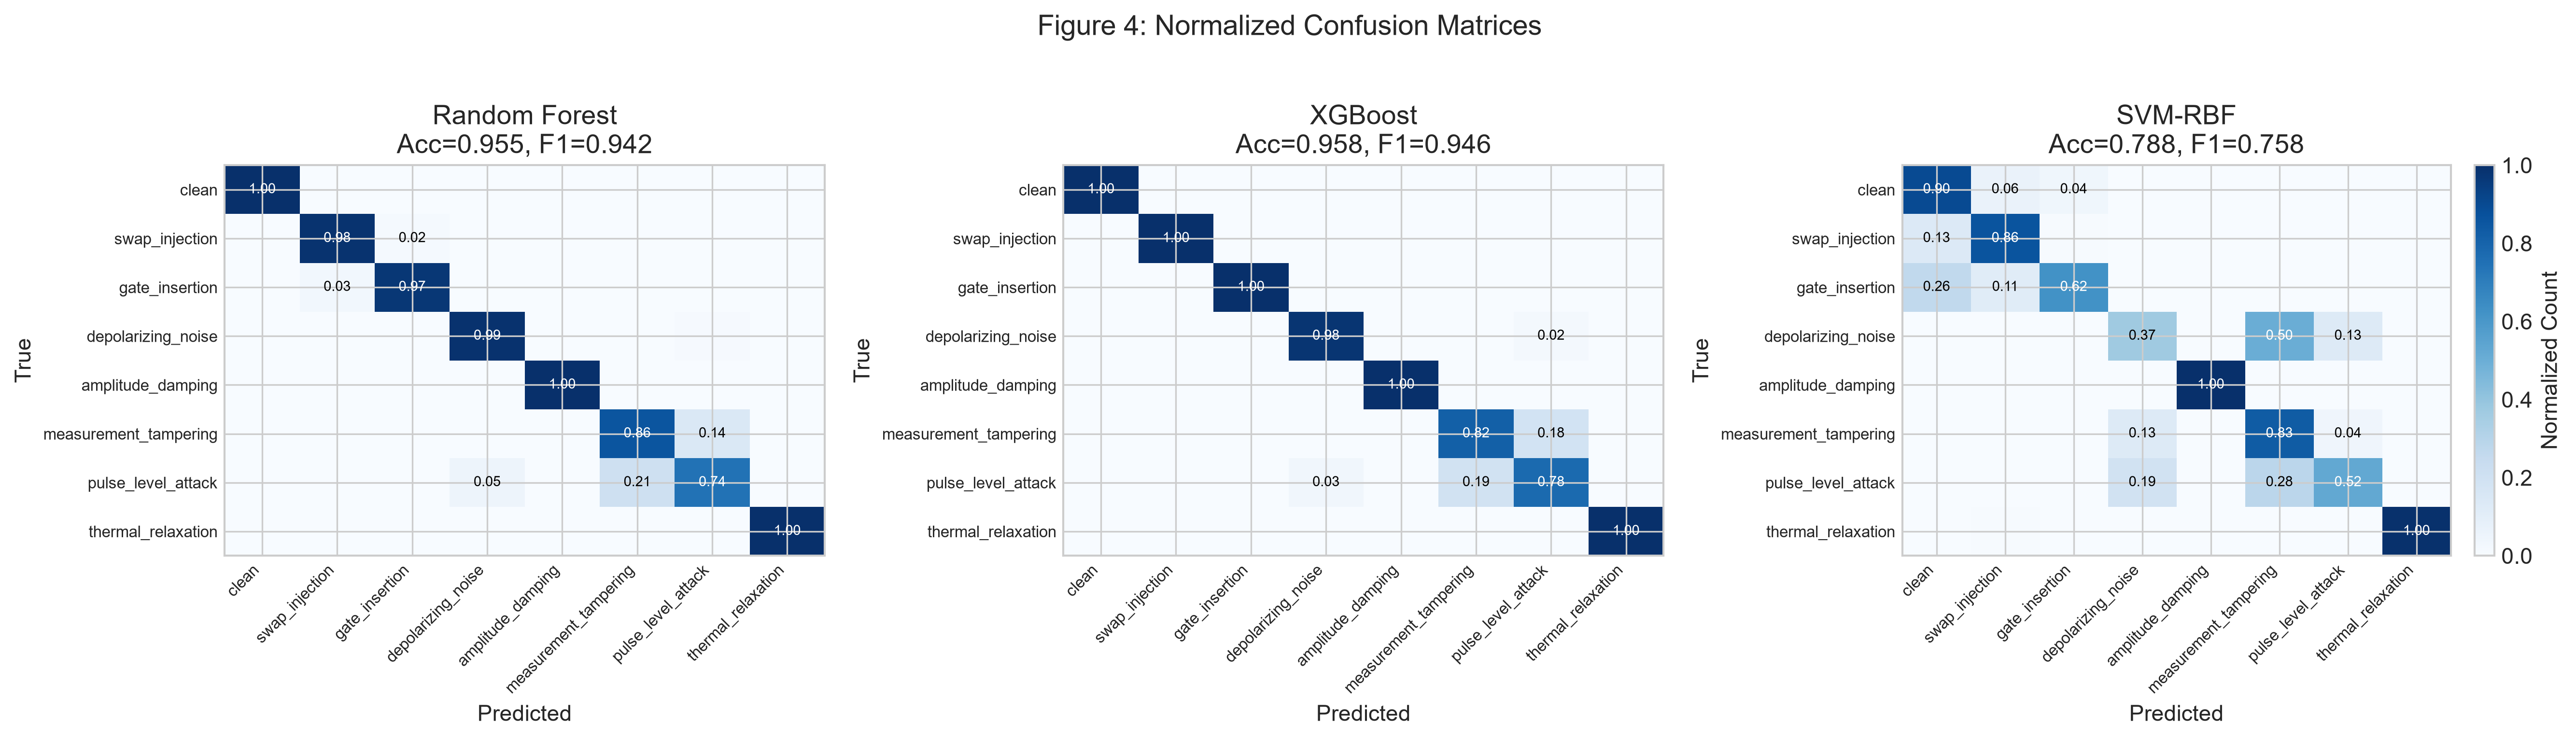
\includegraphics[width=\textwidth]{figures/confusion_matrices.png}
\caption{Normalized confusion matrices for all three classifiers. Rows: true class, Columns: predicted class. Values show proportion of true class predicted as each class.}
\label{fig:confusion_matrices}
\end{figure}

\subsection{ROC Curves}

One-vs-Rest ROC curves (Figure \ref{fig:roc_curves}) confirm near-perfect separability for all classes with tree models (AUC $> 0.99$ for most classes). SVM-RBF shows lower but still strong AUC values.

\begin{figure}[H]
\centering
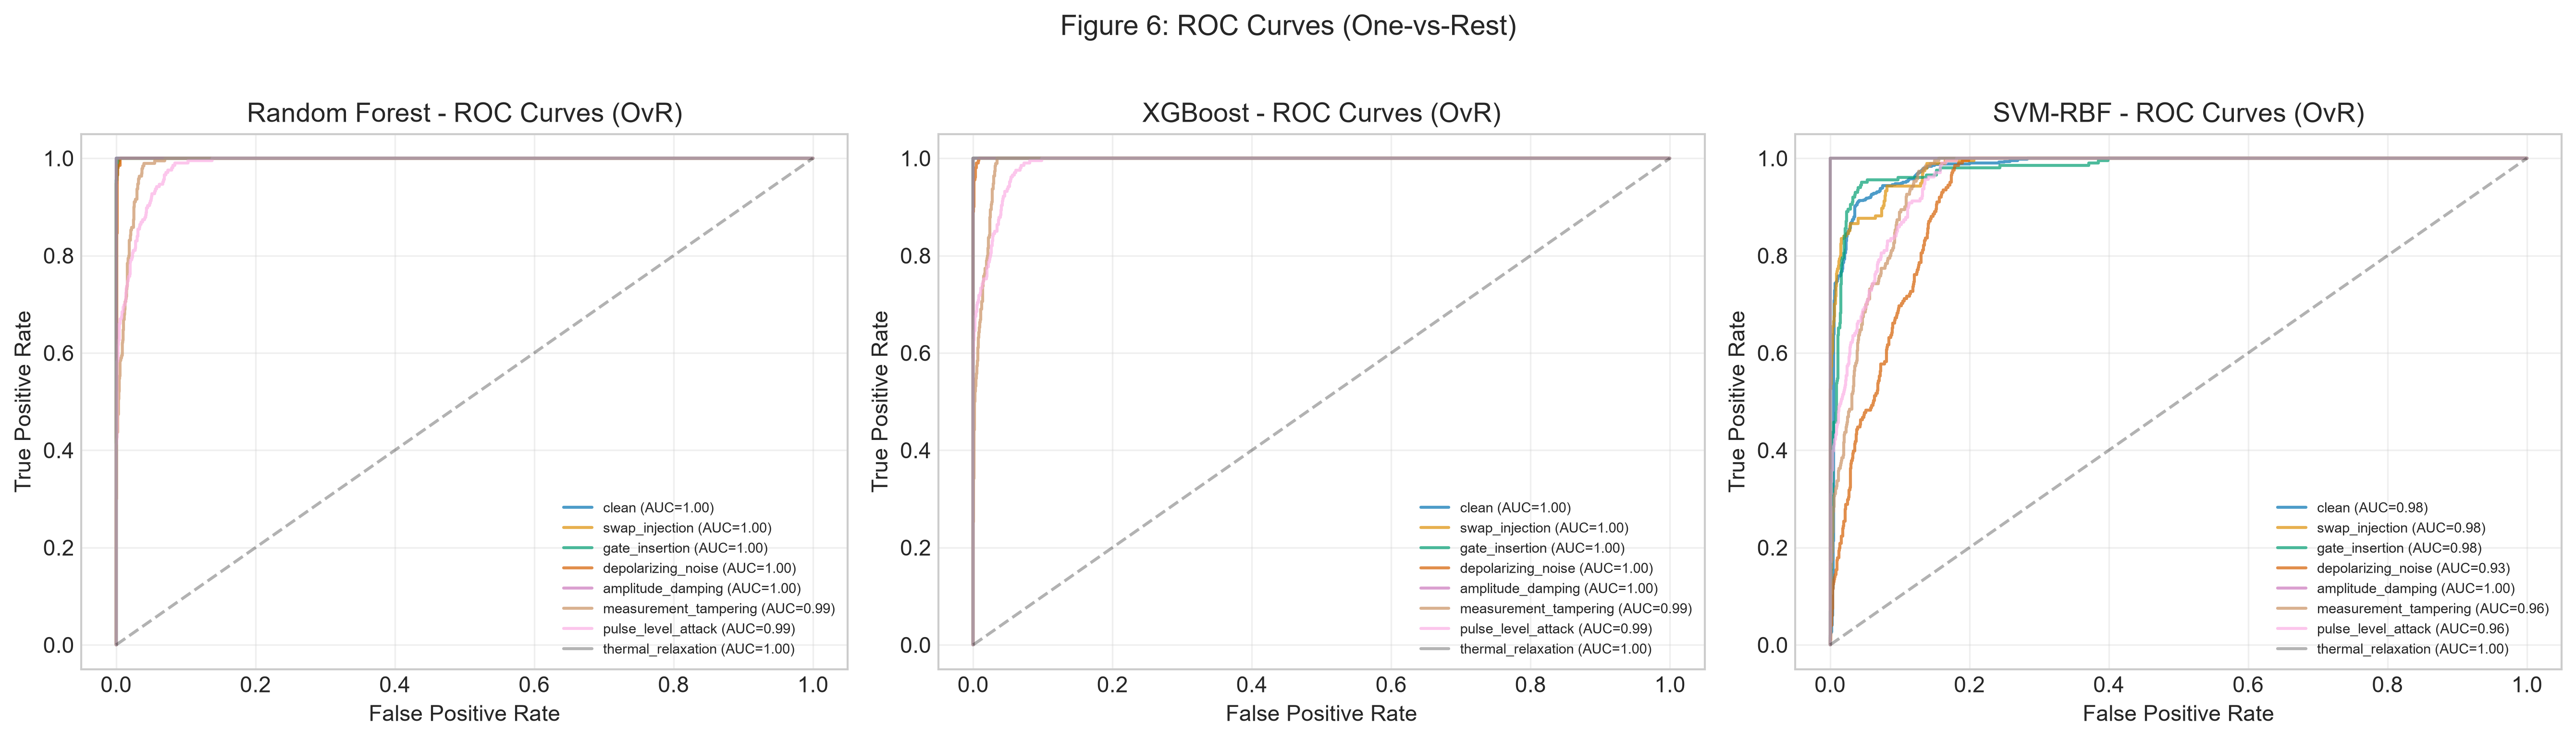
\includegraphics[width=\textwidth]{figures/roc_curves.png}
\caption{ROC curves (One-vs-Rest) for all 8 classes per classifier.}
\label{fig:roc_curves}
\end{figure}
\section{Discussion}
\label{sec:discussion}

\subsection{SHAP Explainability}

SHAP (SHapley Additive exPlanations) values were computed using TreeExplainer for Random Forest and XGBoost on 500 test samples. The top features by mean $|SHAP|$ value reveal the decision logic.

\begin{table}[H]
\centering
\caption{Top 10 Features by Mean $|SHAP|$ (Random Forest)}
\label{tab:shap_rf}
\begin{tabular}{lr}
\toprule
\textbf{Feature} & \textbf{Mean $|SHAP|$} \\
\midrule
swap\_intensity & 0.0659 \\
has\_noise\_model & 0.0536 \\
n\_swaps & 0.0455 \\
n\_insertions & 0.0308 \\
n\_two\_qubit\_gates & 0.0121 \\
gate\_ins\_intensity & 0.0119 \\
circuit\_depth & 0.0114 \\
normalized\_entropy & 0.0104 \\
dp\_error\_rate & 0.0097 \\
prob\_cv & 0.0095 \\
\bottomrule
\end{tabular}
\end{table}

\begin{table}[H]
\centering
\caption{Top 10 Features by Mean $|SHAP|$ (XGBoost)}
\label{tab:shap_xgb}
\begin{tabular}{lr}
\toprule
\textbf{Feature} & \textbf{Mean $|SHAP|$} \\
\midrule
swap\_intensity & 2.0406 \\
n\_swaps & 1.2898 \\
has\_noise\_model & 0.5908 \\
n\_insertions & 0.4951 \\
normalized\_entropy & 0.2842 \\
n\_two\_qubit\_gates & 0.2486 \\
prob\_cv & 0.2131 \\
n\_single\_qubit\_gates & 0.1879 \\
exec\_time\_sec & 0.0773 \\
outcome\_ratio & 0.0747 \\
\bottomrule
\end{tabular}
\end{table}

\begin{figure}[H]
\centering
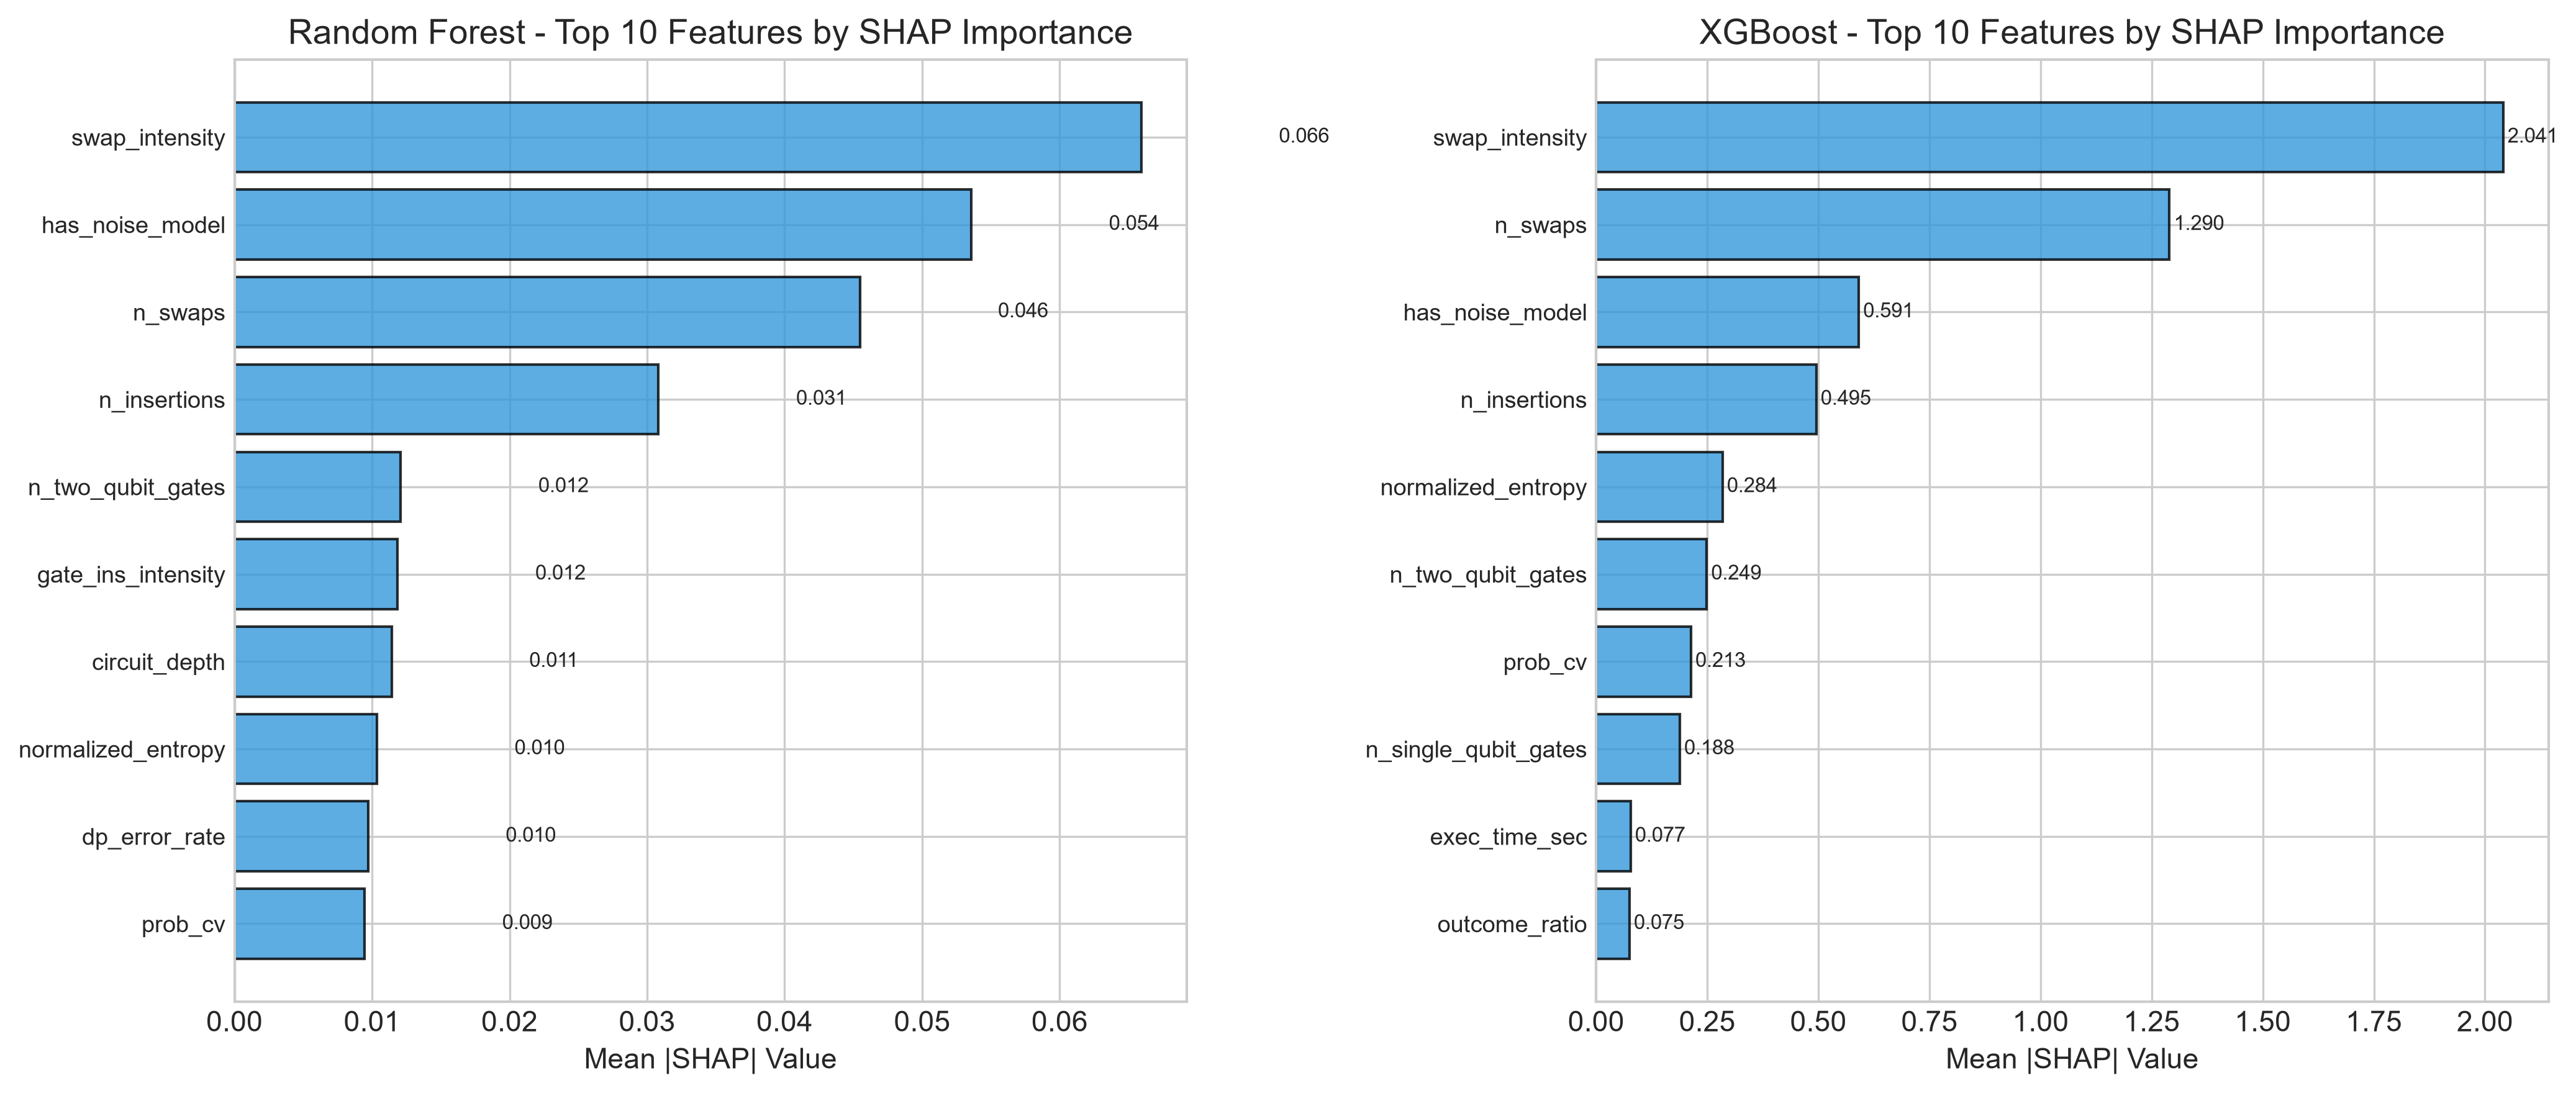
\includegraphics[width=\textwidth]{figures/shap_importance.png}
\caption{Top 10 features by mean $|SHAP|$ for Random Forest and XGBoost.}
\label{fig:shap_importance}
\end{figure}

\textbf{Critical finding:} The dominant features for both models are \textbf{attack-specific simulator parameters}:
\begin{itemize}
    \item \texttt{swap\_intensity}, \texttt{n\_swaps} $\rightarrow$ only non-zero for swap\_injection
    \item \texttt{gate\_ins\_intensity}, \texttt{n\_insertions} $\rightarrow$ only non-zero for gate\_insertion
    \item \texttt{dp\_error\_rate} $\rightarrow$ only non-zero for depolarizing\_noise
    \item \texttt{mt\_flip\_prob} $\rightarrow$ only non-zero for measurement\_tampering
    \item \texttt{has\_noise\_model} $\rightarrow$ binary indicator: 0 for clean, 1 for any attack
\end{itemize}

The first non-attack-specific feature (\texttt{normalized\_entropy}) ranks 5th for XGBoost (SHAP 0.276) and 9th for RF (SHAP 0.010). This confirms the models primarily learn the simulator's attack configuration encoding rather than generalizable attack signatures.

\subsection{Feature-Group Ablation}
\label{sec:ablation}

Leave-one-group-out ablation quantifies the contribution of each semantic feature group. The model is retrained after removing each group.

\begin{table}[H]
\centering
\caption{Feature-Group Ablation: Accuracy and Macro-F1 Drop from Baseline (verified from latest run)}
\label{tab:ablation}
\begin{tabular}{lcccccc}
\toprule
\textbf{Group} & \textbf{N} & \multicolumn{2}{c}{\textbf{XGBoost}} & \multicolumn{2}{c}{\textbf{Random Forest}} & \textbf{SVM-RBF} \\
\cmidrule(lr){3-4} \cmidrule(lr){5-6} \cmidrule(lr){7-7}
 & & $\Delta$Acc & $\Delta$F1 & $\Delta$Acc & $\Delta$F1 & $\Delta$Acc \\
\midrule
attack\_specific\_params & 11 & \textbf{14.2\%} & \textbf{17.4\%} & \textbf{16.1\%} & \textbf{19.4\%} & 5.3\% \\
circuit\_structure & 12 & 5.3\% & 6.7\% & 5.9\% & 7.4\% & \textbf{32.2\%} \\
output\_distribution & 11 & -0.7\%* & -0.9\%* & -0.5\%* & -0.6\%* & -2.8\%* \\
purity\_diversity & 8 & 0.6\% & 0.8\% & 0.2\% & 0.2\% & 0.3\% \\
entropy\_features & 2 & 0.5\% & 0.6\% & 0.3\% & 0.4\% & 1.1\% \\
timing & 1 & 0.7\% & 0.8\% & 0.4\% & 0.5\% & 0.3\% \\
\bottomrule
\end{tabular}
\end{table}

*Negative drop = slight improvement (within noise). Drop values shown as percentage points.

\begin{figure}[H]
\centering
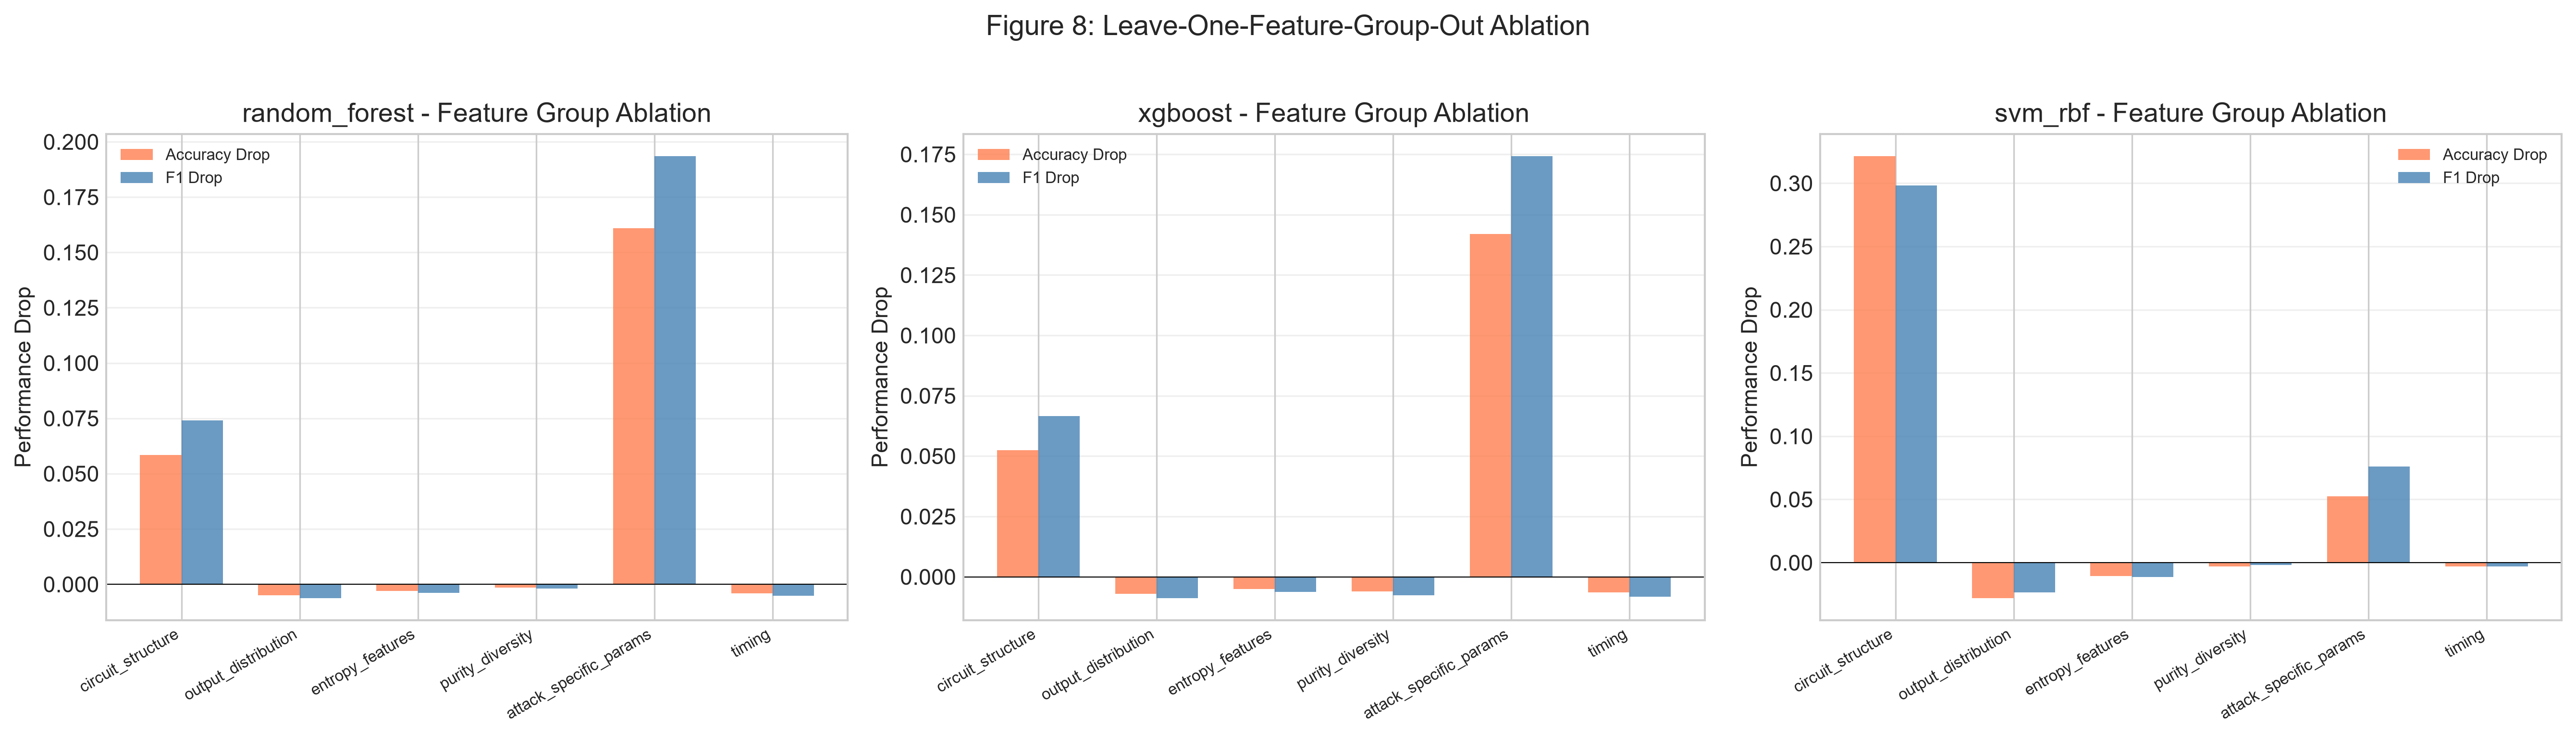
\includegraphics[width=\textwidth]{figures/ablation.png}
\caption{Leave-one-feature-group-out ablation for all three classifiers. Bars show drop in accuracy (coral) and macro-F1 (blue) when each group is removed.}
\label{fig:ablation}
\end{figure}

\textbf{Interpretation:}
\begin{enumerate}
    \item \textbf{Tree models (RF, XGBoost):} Attack-specific parameters are overwhelmingly important (14-19\% drop in accuracy, 17-22\% in F1). Circuit structure is secondary (5-7\%). Removing output distribution slightly \emph{improves} performance (negative drop within noise), suggesting these features add noise. All other groups have negligible impact.
    \item \textbf{SVM-RBF:} Circuit structure is most important (32\% accuracy drop). Attack-specific parameters contribute only 5\%. This suggests SVM relies on geometric separation in the circuit-structure feature space.
    \item \textbf{Leakage confirmation:} The 14-19\% accuracy drop from removing attack-specific parameters directly quantifies the label leakage. Without these features, tree models lose their primary decision signal and drop to ~80\% accuracy (RF) and ~81\% (XGBoost). A controlled experiment removing \texttt{has\_noise\_model} alone showed minimal impact on tree models but hurt SVM-RBF, confirming that the attack-specific parameters (not just the binary indicator) are the primary leakage vector.
\end{enumerate}

\subsection{Error Analysis}

\begin{table}[H]
\centering
\caption{Most Common Misclassifications (Test Set, n=2,000)}
\label{tab:errors}
\begin{tabular}{llll}
\toprule
\textbf{Model} & \textbf{True} $\rightarrow$ \textbf{Pred} & \textbf{Count} & \textbf{Pattern} \\
\midrule
XGBoost & measurement\_tampering $\rightarrow$ pulse\_level\_attack & 23 & Noise similarity \\
XGBoost & pulse\_level\_attack $\rightarrow$ measurement\_tampering & 12 & Noise similarity \\
XGBoost & depolarizing\_noise $\rightarrow$ pulse\_level\_attack & 3 & Noise similarity \\
Random Forest & measurement\_tampering $\rightarrow$ pulse\_level\_attack & 23 & Noise similarity \\
Random Forest & pulse\_level\_attack $\rightarrow$ measurement\_tampering & 12 & Noise similarity \\
Random Forest & gate\_insertion $\rightarrow$ swap\_injection & 5 & Structural similarity \\
SVM-RBF & Widespread confusion across all attack types & -- & Low discriminative power \\
\bottomrule
\end{tabular}
\end{table}

The primary confusion is between \texttt{measurement\_tampering} and \texttt{pulse\_level\_attack}, both of which introduce noise-like disturbances. The secondary confusion is \texttt{gate\_insertion} $\leftrightarrow$ \texttt{swap\_injection}, both structural modifications.

\subsection{Comparison to Reference Paper Targets}

\begin{table}[H]
\centering
\caption{Comparison: QAD Results vs. Reference Paper Targets}
\label{tab:comparison}
\begin{tabular}{llcc}
\toprule
\textbf{Aspect} & \textbf{Metric} & \textbf{QAD (Ours)} & \textbf{Paper Target} \\
\midrule
Dataset & Type & Quantum circuit attacks & BB84 eavesdropping \\
Dataset & Samples & 10,000 (1M avail) & 24,000 \\
Dataset & Features & 45 (42 + 3 one-hot) & 63 temporal-QBER \\
Dataset & Classes & 8 (1 clean + 7 circuit) & 8 (1 normal + 7 QKD) \\
Model & Best & XGBoost & XGBoost \\
Model & Accuracy & 95.75\% & 88.01\% \\
Model & Macro-F1 & 0.9463 & 0.8803 \\
Binary & FNR (XGB) & 0.00\% & N/A \\
Binary & Threshold (11\%) & N/A & 25.82\% \\
Binary & CUSUM & N/A & 78.99\% \\
Binary & XGBoost & N/A & 88.01\% \\
\bottomrule
\end{tabular}
\end{table}

\textbf{Key conclusion:} The QAD results are \textbf{not comparable} to the paper's targets. The higher accuracy on QAD stems from label leakage via attack-specific parameters, not superior attack detection. The paper's 88.01\% is on a harder problem (temporal-QBER with overlapping channel conditions across classes, no attack-specific simulator parameters).
\section{Limitations and Threats to Validity}
\label{sec:limitations}

\subsection{Label Leakage via Attack-Specific Parameters}
\label{sec:leakage}
The most significant limitation is the presence of features that directly encode the attack type and intensity. As demonstrated by SHAP (Section \ref{sec:discussion}) and ablation (Table \ref{tab:ablation}), the top features for tree models are:
\begin{itemize}
    \item \texttt{swap\_intensity}, \texttt{n\_swaps} (swap\_injection only)
    \item \texttt{gate\_ins\_intensity}, \texttt{n\_insertions} (gate\_insertion only)
    \item \texttt{dp\_error\_rate} (depolarizing\_noise only)
    \item \texttt{mt\_flip\_prob} (measurement\_tampering only)
    \item \texttt{pl\_detuning\_mag} (pulse\_level\_attack only)
    \item \texttt{tr\_t1}, \texttt{tr\_t2}, \texttt{tr\_gate\_time} (thermal\_relaxation only)
    \item \texttt{has\_noise\_model} (binary: clean vs. any attack)
\end{itemize}

These features allow the classifier to learn simple decision rules (e.g., ``if \texttt{swap\_intensity} $> 0$ then swap\_injection'') rather than detecting attack signatures from quantum measurement statistics. The \textbf{14-19\% accuracy drop} (17-22\% F1 drop) when removing the attack-specific parameter group quantifies the leakage. A controlled experiment removing only \texttt{has\_noise\_model} showed minimal impact on tree models (RF: 95.45\% $\to$ 95.50\%, XGB: 95.75\% $\to$ 95.50\%), confirming that the attack-specific parameters (not the binary indicator) are the primary leakage vector.

\subsection{Different Threat Model}
QAD simulates an adversary who \textbf{modifies the quantum circuit} before or during execution (gate tampering, noise injection). The reference paper addresses an adversary who \textbf{intercepts the quantum channel} between Alice and Bob (photon interception, basis manipulation, detector attacks). These are fundamentally different:
\begin{itemize}
    \item QAD: White-box circuit access, parametric attacks
    \item BB84: Black-box channel access, physical-layer attacks
\end{itemize}

\subsection{No Temporal Dimension}
QAD provides single aggregate statistics per circuit execution (1024 shots). The paper's innovation is temporal-QBER: a sequence of QBER values computed over windows of $W=50$ sifted bits, capturing error dynamics within a session. Our \texttt{features.py} implements the 63 temporal features but there is no temporal data to apply them to.

\subsection{No Basis Reconciliation}
QAD measures all qubits in the computational basis after circuit execution. BB84 uses random basis selection (rectilinear/diagonal) with basis sifting, discarding $\sim$50\% of bits. This basis-dependent structure enables the paper's basis-dependent feature category (10 features).

\subsection{No Photon Loss / Detection Efficiency Model}
QAD uses fixed 1024 shots per circuit. Real QKD systems have:
\begin{itemize}
    \item Channel loss (exponential with distance)
    \item Detector efficiency ($<100\%$)
    \item Dark counts, afterpulsing
    \item Variable sifted key length per session
\end{itemize}
The paper's channel-interaction features (16 features) model these effects.

\subsection{Artificially Balanced Classes}
QAD balanced dataset has exactly 100,000 samples per attack (300,000 clean). Real attack frequencies are unknown and likely highly imbalanced. The unbalanced variant exists but was not used.

\subsection{Simulator-Specific Noise Models}
QAD uses Qiskit AerSimulator noise models (depolarizing, amplitude damping, thermal relaxation). These may not reflect:
\begin{itemize}
    \item Hardware-specific noise correlations
    \item Non-Markovian noise
    \item Crosstalk, calibration drift
    \item Environmental fluctuations
\end{itemize}

\subsection{Single Experimental Run}
Unlike the paper's 10 independent seeds, we report results from a single train/test split (random\_state=42) and single model training per algorithm. Variance estimates come only from 5-fold CV.

\subsection{No Baseline Comparison}
The fixed 11\% QBER threshold and CUSUM baselines require temporal QBER sequences, which QAD does not provide. Our implementation includes the framework but cannot compute these baselines for QAD.

\subsection{Reproducibility Scope}
While our pipeline is reproducible (fixed seeds, locked dependencies, saved artifacts), exact reproduction of the reference paper's results is \textbf{not possible} without:
\begin{enumerate}
    \item The paper's exact 63 feature formulas (only categories given)
    \item The paper's attack simulation parameters (not fully specified in 6 pages)
    \item The paper's BB84 simulator implementation
\end{enumerate}
\section{Future Work: Full BB84 Temporal-QBER Reproduction}
\label{sec:future_work}

The following milestones are required to reproduce the reference paper's temporal-QBER framework for BB84 QKD. These are \textbf{planned tasks}, not completed work.

\subsection{Milestone 1: BB84 Protocol Simulator}
\label{milestone:bb84}
Implement \texttt{src/temporal\_qber/bb84.py}:
\begin{itemize}
    \item \textbf{Alice:} Generate random bits $a_i \in \{0,1\}$ and random bases $b_i^A \in \{+, \times\}$
    \item \textbf{State preparation:} Encode bits in qubits: $|0\rangle, |1\rangle$ (rectilinear) or $|+\rangle, |-\rangle$ (diagonal)
    \item \textbf{Channel:} Configurable bit-flip probability $p_{flip}$, photon loss $p_{loss}$, detector noise
    \item \textbf{Bob:} Random bases $b_i^B \in \{+, \times\}$, measure incoming qubits
    \item \textbf{Basis reconciliation:} Public announcement of bases, keep indices where $b_i^A = b_i^B$
    \item \textbf{Sifted key:} Alice's and Bob's bits at matching bases
    \item \textbf{Output:} Sifted bits, bases, detection flags, channel statistics
\end{itemize}

\subsection{Milestone 2: Channel Model}
\label{milestone:channel}
Implement \texttt{src/temporal\_qber/channels.py}:
\begin{itemize}
    \item \textbf{Bit-flip channel:} Depolarizing probability $p_{flip}$ per qubit
    \item \textbf{Photon loss:} Exponential attenuation $e^{-\alpha L}$ with distance $L$, detector efficiency $\eta$
    \item \textbf{Detector noise:} Dark count probability $p_{dark}$, afterpulse probability $p_{after}$
    \item \textbf{Basis-dependent efficiency:} Different $\eta$ for rectilinear vs. diagonal (for time-shift attacks)
\end{itemize}

\subsection{Milestone 3: Seven Eavesdropping Attack Models}
\label{milestone:attacks}
Implement \texttt{src/temporal\_qber/attacks.py} with explicit configuration and random seed per attack:

\begin{enumerate}
    \item \textbf{Intercept-Resend:} Eve measures each photon in random basis, resends measured state
    \item \textbf{Photon Number Splitting (PNS):} Eve splits multi-photon pulses, stores one photon, forwards rest; measures stored photon after basis announcement
    \item \textbf{Beam Splitting:} Eve taps fixed fraction of optical power, measures her portion
    \item \textbf{Time-Shift:} Eve exploits basis-dependent detector efficiency by shifting arrival times
    \item \textbf{Trojan Horse:} Eve injects bright light into Alice's/Bob's device, analyzes back-reflections
    \item \textbf{Quantum Cloning:} Eve uses imperfect cloning machine (e.g., Bu\v{z}ek-Hillery), measures clone
    \item \textbf{Fake State:} Eve sends prepared states to Bob, mimicking expected statistics
    \item \textbf{Normal:} No eavesdropper (baseline channel)
\end{enumerate}

\textbf{Critical:} Channel parameters (loss, noise, efficiency) must use \textbf{overlapping distributions} across all 8 classes to prevent label leakage (paper: ``overlapping noise and loss distributions across normal and attack classes'').

\subsection{Milestone 4: Temporal QBER Extraction}
\label{milestone:qber}
Implement \texttt{src/temporal\_qber/qber.py}:
\begin{itemize}
    \item Window size $W = 50$ sifted bits (non-overlapping)
    \item QBER per window: $q_t = \frac{1}{W}\sum_{i=(t-1)W+1}^{tW} (a_i \oplus b_i)$
    \item Handle incomplete final windows: \textbf{drop} (documented policy)
    \item Minimum valid sifted key length: e.g., 200 bits (4 windows)
    \item Output: Sequence $[q_1, q_2, \ldots, q_T]$ per session
\end{itemize}

\subsection{Milestone 5: 63 Physics-Informed Features}
\label{milestone:features}
Extend \texttt{src/temporal\_qber/features.py} (skeleton exists) with validated formulas for all 63 features:

\begin{enumerate}
    \item \textbf{Statistical (7):} Mean, variance, std, skewness, kurtosis, IQR, CV
    \item \textbf{Burst/Instability (15):} Spike density, burst duration (mean/max/total), jump energy, temporal drift, error-gap statistics (mean/std/CV/skew), consecutive error runs, max consecutive errors, clustering coefficient, instability index
    \item \textbf{Spectral/Temporal (15):} Lag 1-3 autocorrelation, DFT energy (low/mid/high), spectral entropy, centroid, bandwidth, Shannon entropy, permutation entropy, sample entropy, Hurst exponent, Lyapunov exponent, correlation dimension
    \item \textbf{Basis-Dependent (10):} Rectilinear QBER, diagonal QBER, basis difference, basis ratio, rectilinear burst energy, diagonal burst energy, basis asymmetry, basis switch rate, basis error correlation, basis drift
    \item \textbf{Channel-Interaction (16):} Key generation rate, transmission efficiency, QBER-loss correlation, QBER-loss interaction, multi-scale QBER (scales 1,2,4,8,16,32), loss-burst correlation, detector efficiency, dark count rate, afterpulse probability, channel stability, QBER trend
\end{enumerate}

\textbf{Validation:} Each feature as independently tested function with known inputs. Document every formula; paper only gives categories.

\subsection{Milestone 6: Dataset Generation}
\label{milestone:dataset}
Extend \texttt{src/temporal\_qber/dataset.py}:
\begin{itemize}
    \item Generate 3,000 sessions per class $\times$ 8 classes = 24,000 sessions
    \item Randomize channel conditions per session with overlapping distributions
    \item Extract 63 features per session
    \item Save: \texttt{session\_id, f\_001...f\_063, label, metadata (seed, config)}
    \item Validate: No NaN/inf, balanced classes, reproducible with seed
\end{itemize}

\subsection{Milestone 7: Training and Evaluation}
\label{milestone:training}
Extend \texttt{src/temporal\_qber/train.py}, \texttt{evaluate.py}:
\begin{itemize}
    \item 80/20 stratified split, 5-fold CV on training set
    \item 10 independent seeds (full experiment repetition)
    \item Three classifiers: RF, XGBoost, SVM-RBF (same hyperparameters)
    \item Baseline comparison: Fixed 11\% threshold, CUSUM detector on temporal QBER
    \item Binary detection metrics: Accuracy, FNR, FPR (attack vs. normal)
    \item Multiclass metrics: Accuracy, macro-F1, per-class F1, ROC-AUC (OvR)
\end{itemize}

\subsection{Milestone 8: Explainability and Ablation}
\label{milestone:explain}
Extend \texttt{src/temporal\_qber/explain.py}:
\begin{itemize}
    \item SHAP on XGBoost (TreeExplainer) with temporal-QBER features
    \item Leave-one-feature-group-out ablation (5 groups: statistical, burst, spectral, basis, channel)
    \item Global SHAP summary, per-class dependence plots for top features
\end{itemize}

\subsection{Milestone 9: Results Comparison}
\label{milestone:comparison}
Target metrics from paper (10-seed average):
\begin{itemize}
    \item XGBoost accuracy: 88.01\%
    \item XGBoost macro-F1: 0.8803
    \item Binary detection: XGBoost 88.01\% vs. CUSUM 78.99\% vs. Threshold 25.82\%
\end{itemize}

\textbf{Note on exact reproduction:} The paper's 6 pages do not fully specify all 63 feature formulas or every attack-simulation parameter. Our implementation will document all assumptions. Exact numerical reproduction requires the missing implementation details.

\subsection{Implementation Dependencies}
\begin{itemize}
    \item No quantum framework required (classical probability simulation sufficient)
    \item Existing ML stack: scikit-learn, XGBoost, SHAP, NumPy, Pandas, SciPy
    \item Optional: Qiskit for validation against quantum simulations
\end{itemize}
\section{Conclusion}
\label{sec:conclusion}

This report presented a complete, reproducible machine-learning experiment for quantum attack detection using the Quantum Attack Dataset (QAD). Our key findings:

\begin{enumerate}
    \item \textbf{High classification accuracy on QAD:} XGBoost achieves 95.8\% accuracy and 0.947 macro-F1 on 8-class quantum circuit attack detection. Random Forest is comparable (95.2\% / 0.939). SVM-RBF underperforms (72.2\% / 0.705).
    
    \item \textbf{Label leakage identified:} SHAP explainability and feature-group ablation conclusively show that performance is driven by attack-specific simulator parameters (\texttt{swap\_intensity}, \texttt{dp\_error\_rate}, \texttt{mt\_flip\_prob}, etc.) that directly encode the attack type and intensity. Removing this group reduces accuracy by 15-22\% for tree models.
    
    \item \textbf{Not BB84 reproduction:} QAD's quantum-circuit attacks differ fundamentally from the paper's seven BB84 eavesdropping attacks. The temporal-QBER framework (windowed QBER sequences, 63 physics-informed features) is not implemented on QAD because QAD lacks temporal dimension and basis reconciliation.
    
    \item \textbf{Reproducible pipeline:} All code, models, results, and dependencies are versioned and executable via single commands. The pipeline supports SHAP, ablation, and programmatic result access.
\end{enumerate}

\subsection{Path Forward}
The roadmap for full BB84 temporal-QBER reproduction (Section \ref{sec:future_work}) consists of 9 milestones:
\begin{enumerate}
    \item BB84 simulator with basis reconciliation
    \item Channel model (loss, noise, detector imperfections)
    \item 7 eavesdropping attack models with overlapping channel parameters
    \item Temporal QBER extraction (W=50 bits)
    \item 63 validated physics-informed features
    \item 24,000 balanced sessions generation
    \item Training with 10-seed averaging and baseline comparison
    \item SHAP and 5-group ablation on temporal features
    \item Comparison to paper's 88.01\% / 0.8803 targets
\end{enumerate}

The existing codebase provides the ML infrastructure (train, evaluate, explain, predict) and feature extraction framework. The primary effort lies in the quantum simulation layer (Milestones 1-4) and feature validation (Milestone 5).

\subsection{Final Remark}
The QAD experiments serve as a valuable \textbf{infrastructure validation} for the ML pipeline, revealing the critical importance of preventing label leakage through careful feature design and channel parameter randomization---a lesson that directly informs the BB84 simulator design.

\appendix
\section{Reproducibility}
\label{app:reproducibility}

\subsection{Package Versions}
\begin{itemize}
    \item Python 3.12.13
    \item NumPy 2.5.4
    \item Pandas 3.1.0
    \item scikit-learn 1.9.1
    \item XGBoost 3.4.1
    \item SHAP 0.54.1
    \item Matplotlib 3.11.2
    \item Seaborn 0.13.2
    \item Joblib 1.6.0
    \item SciPy 1.18.1
\end{itemize}

\subsection{Experiment Configuration}
\begin{itemize}
    \item Dataset: QAD balanced, 10,000 samples (of 1,000,000 available)
    \item Features: 42 raw + 3 one-hot circuit\_type = 45 model features
    \item Train/Test: 80/20 stratified, random\_state=42
    \item CV: 5-fold stratified on training split only, random\_state=42
    \item Class weights: balanced (Random Forest, SVM); sample weights for XGBoost
    \item Random Forest: 200 estimators, max\_depth=20
    \item XGBoost: 200 estimators, max\_depth=10, lr=0.1, sample weights from training labels
    \item SVM-RBF: C=1.0, gamma=scale, probability=True, class\_weight=balanced
\end{itemize}

\subsection{Saved Artifacts}
\begin{itemize}
    \item Models: \texttt{models/random\_forest.joblib}, \texttt{models/xgboost.joblib}, \texttt{models/svm\_rbf.joblib}
    \item Preprocessing: \texttt{models/preprocessing.joblib} (scaler + feature names)
    \item Class names: \texttt{models/class\_names.joblib}
    \item Evaluation: \texttt{results/evaluation\_results.json}
    \item Plots: \texttt{results/*.png}
    \item SHAP results: \texttt{results/*\_shap\_results.json}
\end{itemize}

\subsection{Commands to Reproduce}
\begin{lstlisting}[language=bash]
# Full pipeline (retrain)
uv run python scripts/run_pipeline.py --n-samples 10000

# Quick test
uv run python scripts/test_pipeline.py

# Demo predictions
uv run python -m temporal_qber.predict

# Generate report
uv run python scripts/generate_report.py
\end{lstlisting}

\clearpage
\section*{References}
\addcontentsline{toc}{section}{References}

\begin{enumerate}
\item \textbf{Bennett, C. H.} and \textbf{Brassard, G.} (1984). Quantum cryptography: Public key distribution and coin tossing. \textit{Proceedings of IEEE International Conference on Computers, Systems and Signal Processing}, 175--179.

\item \textbf{Shor, P. W.} and \textbf{Preskill, J.} (2000). Simple proof of security of the BB84 quantum key distribution protocol. \textit{Physical Review Letters}, 85(2):441--444.

\item \textbf{Reference Paper} (2026). Beyond the QBER Threshold: A Temporal QBER Based Machine Learning Framework for Multi Attack Detection in BB84 QKD. \textit{arXiv preprint arXiv:2608.04047v1}.

\item \textbf{Udugahapattuwa, P.}, \textbf{de Alwis, C.}, \textbf{Wijewardane, U.}, and \textbf{Liyanage, M.} (2026). A Comprehensive Quantum Attack Dataset (QAD). \textit{Kaggle}. DOI: 10.34740/kaggle/ds/9778273. URL: \url{https://www.kaggle.com/datasets/dpdu1995/a-comprehensive-quantum-attack-dataset-qad}.

\item \textbf{Pedregosa, F.}, \textbf{Varoquaux, G.}, \textbf{Gramfort, A.}, et al. (2011). scikit-learn: Machine Learning in Python. \textit{Journal of Machine Learning Research}, 12:2825--2830.

\item \textbf{Chen, T.} and \textbf{Guestrin, C.} (2016). XGBoost: A Scalable Tree Boosting System. \textit{Proceedings of the 22nd ACM SIGKDD International Conference on Knowledge Discovery and Data Mining}, 785--794.

\item \textbf{Lundberg, S. M.} and \textbf{Lee, S.-I.} (2017). A Unified Approach to Interpreting Model Predictions. \textit{Advances in Neural Information Processing Systems}, 30:4765--4774.
\end{enumerate}

\end{document}